%\section{Reconstruction and Scalability of Coordinate Descent}
%\textbf{Coordinate Descent comparison to CLEAN reconstruction}
\section{Coordinate Descent Reconstructions on Simulated Data}
In this section, we compare the Coordinate Descent reconstruction with CLEAN on simulated MeerKAT data, and compare the runtime complexity of the two approaches on a real-world MeerKAT observation. We show that Coordinate Descent reconstructs the image by only computing a subset  the Fourier Transform Matrix' columns $F^{-1}$, and investigate if this approach reduces the runtime complexity on the large scale reconstruction problems of MeerKAT.

The real world MeerKAT data were calibrated and averaged down to reduce its size to 88 Gigabytes. The raw, uncalibrated data ranges between 500 and 1000 Gigabytes. Data on this scale requires a mature pipeline for reading and image reconstruction. Within the time limit of this project, only a reconstruction with the WSCLEAN\cite{offringa2014wsclean} pipeline was possible.

The simulations were created with the Meqtrees software package. Two simulations which contain roughly (size of Visibilities) perfectly calibrated Visibilities were created. Compared to real-world observations, the two simulated data sets are small and not representative of the real data volume. Also, more realistic simulations which contain pointing errors, calibration errors, and thermal noise are out of scope for this project. The simulations are used to isolate the two fundamental issues in radio interferometer image reconstruction: Non-uniform sampling and incomplete measurements.

\subsection{Imaging on Simulated Data}
We compare the reconstruction of Coordinate Descent and CLEAN on two simulated observations. The first observation contains two point sources, on which we show that Coordinate Descent is able to locate the sources below the accuracy limit of the instrument. The second observation contains point and Gaussian sources, on which we show that Coordinate Descent better captures the intensity profile of extended emissions. Also, we look at the shortcomings of the proof-of-concept implementations in terms of reconstruction quality and runtime. We use the CLEAN implementation of CASA in this section. CASA is an established software framework for radio interferometer image reconstruction and was already used in a previous project.

\begin{figure}[h]
	\centering
	\begin{subfigure}[b]{0.4\linewidth}
		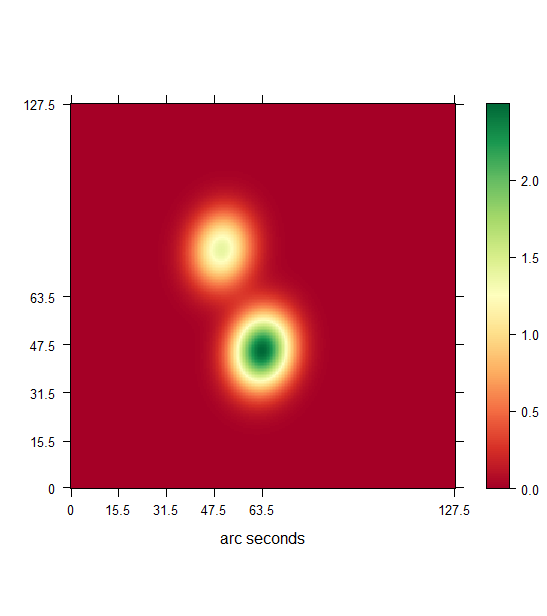
\includegraphics[width=\linewidth]{./chapters/20.results/points/tCLEAN.png}
		\caption{CLEAN reconstruction.}
		\label{results:points:tclean}
	\end{subfigure}
	\begin{subfigure}[b]{0.4\linewidth}
		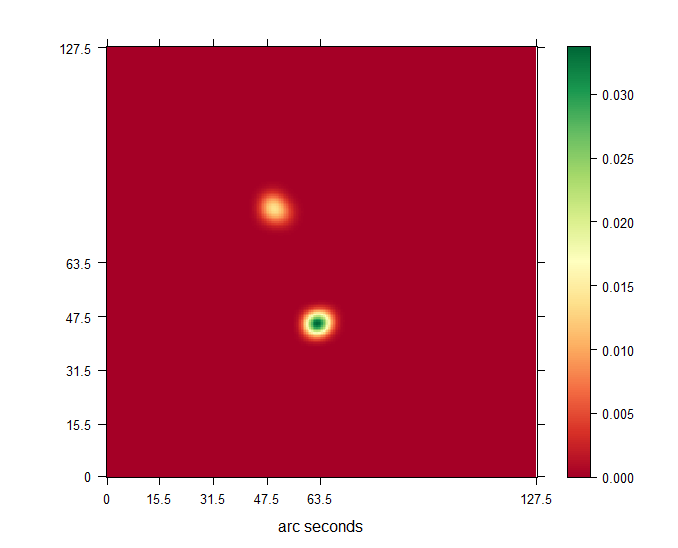
\includegraphics[width=\linewidth]{./chapters/20.results/points/cd.png}
		\caption{Coordinate Descent reconstruction.}
		\label{results:points:cd}
	\end{subfigure}
	
	\caption{Image reconstruction of two point sources.}
	\label{results:point}
\end{figure}

We used CASA's default parameters for CLEAN, except for the maximum number of CLEAN iterations, which we set to 250. The proof-of-concept Coordinate Descent implementation has three parameters to tune: Number of iterations, the number of starlet layers $J$, and the regularization parameter $\lambda$. The first two parameter could be estimated by the reconstruction algorithm itself. In this implementation, it was left to the user. For the two simulations the Coordinate Descent parameters were chosen:
\begin{itemize}
	\item Two Point sources: 4 full iterations, $J=3$, $\lambda=0.1$
	\item Mixed sources: 4 full iterations, $J=7$, $\lambda=0.1$
\end{itemize}

In figure \ref{results:point} shows an image of the Coordinate Descent and CLEAN reconstruction. Figure \ref{results:points:contour} shows the intensity profile of both reconstructions compared with the ground truth. Note that figure \ref{results:points:contour} has a logarithmic y axis. The reconstructions differ in two notable ways: The peak intensity of the source, and how much each algorithm spreads the point source. 

\textit{Spread}: CLEAN reconstructs a convolved version of the true image. CLEAN locates the two peaks in figure \ref{results:points:contour}, but convolves the point source with a Gaussian function. CLEAN reconstructs two Gaussian functions with same peak as the point source. The Gaussian represents the accuracy of the instrument. With compressed sensing, we try to reconstruct the observed image above the accuracy of the instrument. In the intensity profile, Coordinate Descent reconstructs two narrow gaussian-like peaks, essentially super-resolving the image. However, note that the total intensity is a fraction of the original peaks.

\textit{Intensity:} [Total Flux] The reconstructions differ in intensity. The figure \ref{results:points:contour} shows the intensity pr. Also note that Coordinate Descent has shifted the smaller peak by a pixel in its reconstruction. [Total flux correct in CD?]

\begin{figure}[h]
	\centering
	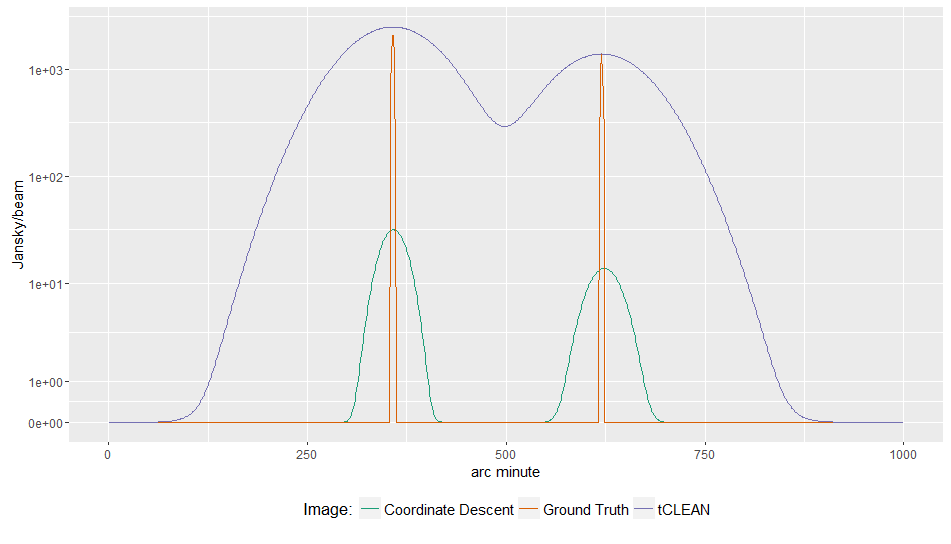
\includegraphics[width=0.8\linewidth]{./chapters/20.results/points/line.png}
	\caption{Intensity profile of the two point sources.}
	\label{results:points:contour}
\end{figure}

The difference in intensity becomes more apparent with extended emissions. Figure \ref{results:mixed} shows Coordinate Descent and tCLEAN on the simulation with mixed sources. Again the two reconstructions arrive at different intensities. The gaussian emissions are reconstructed with a higher intensity than Coordinate Descent.

\begin{figure}[h]
	\centering
	\begin{subfigure}[b]{0.4\linewidth}
		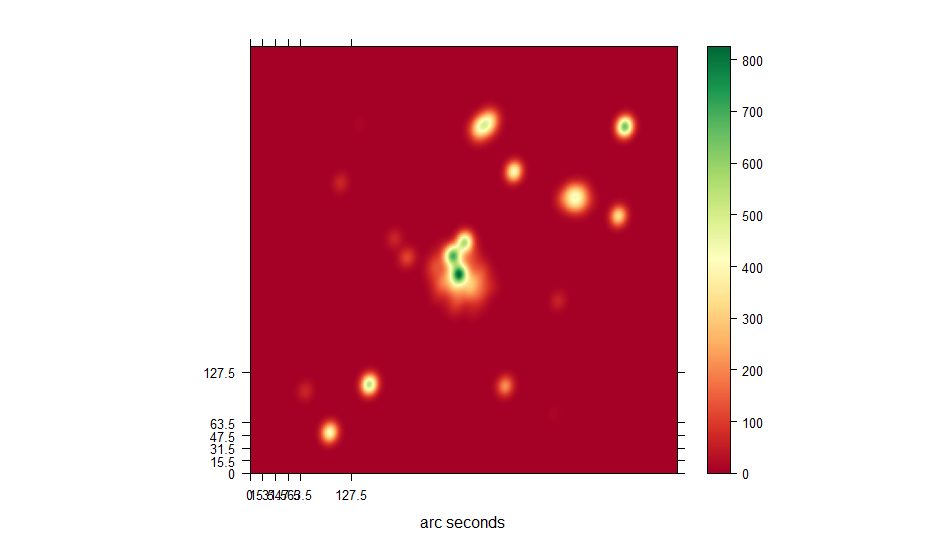
\includegraphics[width=\linewidth]{./chapters/20.results/mixed/mixed_tclean.png}
		\caption{tclean reconstruction}
		\label{results:mixed:tclean}
	\end{subfigure}
	\begin{subfigure}[b]{0.4\linewidth}
		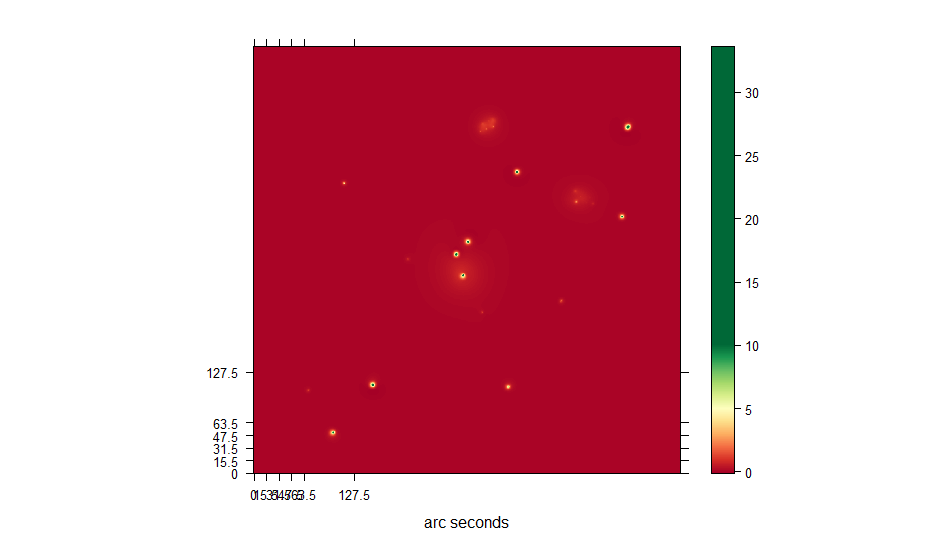
\includegraphics[width=\linewidth]{./chapters/20.results/mixed/mixed_cd.png}
		\caption{Coordinate Descent Reconstruction}
		\label{results:mixed:cd}
	\end{subfigure}
	\caption{Reconstruction on mixed sources}
	\label{results:mixed}
\end{figure}

With starlets, coordinate descent has a representation for extended emissions. Looking at the intensity profile of an extended emisions \ref{}, we see Coordiante Descent coming closer to the true intensity. Although in the four iterations,  [it still had a considerable margin on error]. 

Total flux constraint, $\lambda$ for different starlet layers like in \cite{girard2015sparse}

Coordinate Descent did not reconstruct all point sources. How many starlets are non-zero is the major point for runtime. It depends on how many areas of the image are non-zero. Starlet has a representation for extended emission, how many starlets are needed for modelling is hard.

Runtime problems
19 non-zero starlets, 


\pagebreak
\section{Runtime complexity on large scale reconstructions}
Pinning down the average runtime of Coordinate Descent is difficult. As mentioned in section \ref{cd}, Coordinate Descent has lose convergence guarantees in theory, but works well in practice with heuristics. For our algorithm, the runtime mainly depends on the number of non-zero starlet components $S$ and how many iterations Coordinate Descent needs to converge. How many non-zero starlets, or how many iterations Coordinate Descent needs on average are hard questions and cannot be answered in this project.

Instead, this work focuses on a minimum runtime estimate of Coordinate Descent on MeerKAT observations. We compare the runtime complexity with CLEAN and analyse what speed up an idealized version of Coordinate Descent can provide. Sadly, the speed up of an idealized Coordinate Descent is negligible. The Major Cycle architecture leads to a lower runtime complexity in the context of MeerKAT reconstructions.


\subsection{Runtime complexity of an idealized Coordinate Descent}
The runtime complexity of Coordinate Descent depends largely on the number of Visibilities $M$ and the number of non-zero starlets $S$. The number and location of the $S$ non-zero starlets are generally not known. However, we created a heuristic which finds likely non-zero starlet components. In a realistic setting, the heuristic will have found more than $S$ likely non-zero starlets. For the best case scenario, we assume an oracle performance heuristic: It finds the location and number of the $S$ non-zero starlet components in constant time ($O(1)$). Coordinate Descent therefore has to find the value of the $S$ non-zero starlet components, which takes three separate operations: creating the columns of $F^{-1}$, calculating the minima for each single component, and calculating the starlet layers:

\begin{alignat*}{1}
\text{creating} \:S\: \text{columns of}\: F^{-1} &: S*7M\\
\text{locating} \:S\: \text{minima of} \:S\: \text{parabolas} &: S*4M\\
\text{calculating} \:J\: \text{Starlet layers} &: J * 2M
\end{alignat*}

We assume we have enough memory to cache the columns of $F^{-1}$ and only need to calculate them once. Coordinate Descent arrives at the correct result in $I_{CD}$ iterations. Therefore we arrive at the runtime complexity of \eqref{results:cd:omega}.

\begin{equation}\label{results:cd:omega}
CD(I_{CD}, M, S, J) = S*7M + I_{CD} * [S * 4M + J * 2M]
\end{equation}

Note that the runtime of Coordinate Descent is independent of the number of pixels. The only image related parameter in \eqref{results:cd:omega} is $J$, the number of starlet layers. The largest starlet layer represents the largest possible structure in the image, which is given by the instrument and the image resolution (pixels per arc-second). The runtime only depends indirectly on the image resolution, not the total number of pixels.

Also note the term iterating over the $S$ non-zero starlets, $ I_{CD} * [S * 4M +\ldots]$. As it turns out, this is the Achilles heel of the algorithm. MeerKAT observations contain a very large amount of Visibilities $M$ and a large amount of distinct structures, which leads to a large $S$ (each point source needs at least one non-zero component to be represented). 

\subsection{Runtime complexity of CLEAN}
We look at CLEAN reconstructions which use the non-uniform FFT with $w$-stacking. The runtime of a single Major cycle depends on the non-uniform FFT with $w$-stacking and the number of CLEAN deconvolutions. The number $N$ denotes the number of pixels (for example $512^2$).

\begin{alignat*}{1}
	\text{non-uniform FFT} &: M + 2N*ld(2N)\\
	\text{non-uniform FFT with} \:w\text{-stacking} &:M + W*(2N*ld(2N) + 2N) + N*ld(N)\\
	I_{CLEAN}\: \text{deconvolutions} &: I_{CLEAN}*2N
\end{alignat*}

The overall complexity shown in \eqref{results:clean:o} can also be split into two parts: It depends on the number of Major on the number of Major Cycles $I_{Major}$ and the complexity of the non-uniform FFT, and $I_{Major}$ times the CLEAN deconvolutions. 

\begin{equation}\label{results:clean:o}
\begin{aligned}
 CLEAN(I_{Major}, I_{CLEAN}, M, N,  W) =\: &I_{Major} * 2 * [M + W*(2N log 2N + 2N) + N log N]\\
+ &I_{Major} * [I_{CLEAN}*2N]
\end{aligned}
\end{equation}

Notice that the number of CLEAN deconvolutions $I_{CLEAN}$ depends on the image content, similar the number of non-zero starlets $S$ for Coordinate Descent. Here however, it multiplies with the number of pixels $N$ instead of the number of Visibilities $M$. In a sense, the major cycle tries to reduce the runtime complexity of handling the image content by calculating the non-uniform FFT. If the difference is large enough $N \ll M$, then the Major Cycle will end up with a smaller overall runtime.


\subsection{Comparison on a MeerKAT reconstruction problem}
The MeerKAT observation contains approximately 540 channels with 4 million calibrated Visibilities each. After calibration, MeerKAT data is typically averaged over frequency and time to reduce its disk space. There are no strict rules on how to chose the image resolution and number of pixels. An initial WSCLEAN reconstruction was preformed with:
\begin{itemize}
	\item Visibilities: $M=2.19e^9$
	\item $w$-stacks: $W = 128$
	\item Pixels: $N = 8192^2$
	\item Maximum number of CLEAN iterations: $I_{CLEAN} = 35'000$
\end{itemize}

For our estimate, we use the values of the initial WSCLEAN reconstruction, and we assume CLEAN requires $I_{Major}=10$ Major Cycles to converge. CLEAN reconstructions tend to use around five Major Cycles. Compressed sensing reconstructions which use the Major Cycle framework tend to use around 10 cycles. For the first estimate, we make assumptions in favour of Coordinate Descent.

The idealized Coordinate Descent algorithm has three parameters left: Number of starlet levels $J$, number of non-zero starlets $S$, and number of iterations to converge $I_{CD}$. We under-estimate and set $J=5$, and assume the largest structure in the image is no more than 160 pixels in size. With these assumptions we plug in the values into the equations \eqref{results:cd:omega} and \eqref{results:clean:o}, and compare the runtime for different values of $S$ and $I_{CD}$ in table \ref{res:cd:table}

\begin{table}[h!]
	\begin{center}
		\begin{tabular}{l|c|c|c|c} % <-- Alignments: 1st column left, 2nd middle and 3rd right, with vertical lines in between
			 & $I_{CD} = 1$ & $I_{CD} = 5$ &  $I_{CD} = 10$ &  $I_{CD} = 15$\\
			\hline
			$S=1000$ & 2.35 & 1.12 & 0.66 & \\
			$S=2000$ & 1.17 & 0.56 & 0.33 &\\
			$S=3000$ & 0.78 & 0.37 & 0.22 &\\
			$S=4000$ & 0.59 & 0.28 & 0.17 & \\
		\end{tabular}
		\caption{Relative speed-up of an idealized Coordinate Descent compared to CLEAN.}
		\label{res:cd:table}
	\end{center}
\end{table}

To put the numbers into perspective, Coordinate Descent used about 2000 non-zero starlets to reconstruct the image \ref{results:mixed:cd}. Since the reconstruction does not contain all point sources, the true number of $S$ is likely to be higher than 2000 on a simulated dataset with simple, Gaussian extended emissions. A MeerKAT reconstruction can contain more complex emissions. Figure \ref{results:wsclean} shows the WSCLEAN reconstruction of the current observation. We see a large number of small, point-like objects and several complex extended emissions. We need at least 2000 non zero starlet components to represent the MeerKAT image. In the best case scenario, when the ideal Coordinate Descent converges within one iteration, we have a 17\% runtime improvement over CLEAN. Keep in mind that we have over-estimated the runtime of CLEAN.

\begin{figure}[h]
	\centering
	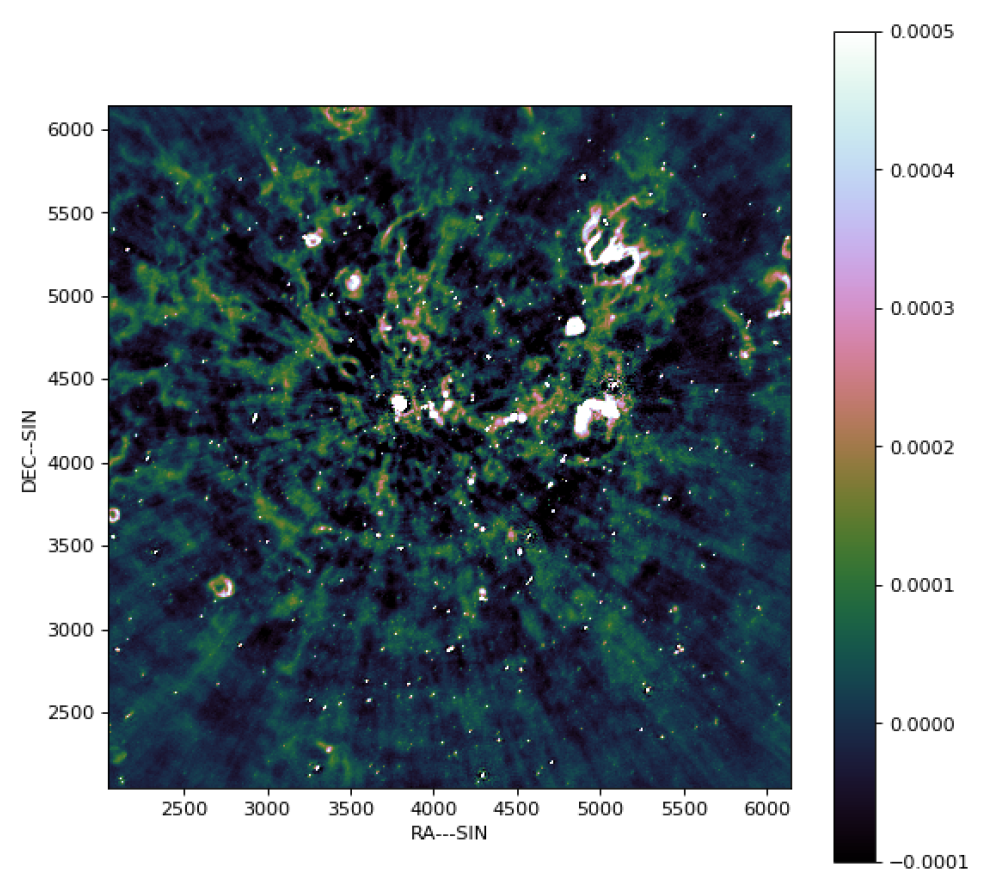
\includegraphics[width=0.6\linewidth]{./chapters/20.results/meerkat.png}
	\caption{WSCLEAN Reconstruction of the MeerKAT observation.}
	\label{results:wsclean}
\end{figure}


Memory


Let us ignore the memory requirement. Coordinate Descent does not scale with the number of pîxels. since this number is typically left to the user, the question remains if Coordinate Descent is worth the costs if we have a lot more pixels. We do a similar estimate, but quadruple each image dimension to $N=32768^2$ and compare the speed up to CLEAN in table \ref{res:cd:large:table}. 

Half as many pixels as Visibilities. An extreme example.


   when we say we need at least $S=2000$, and at least as many iterations for reconstruction. Since Coordinate Descent does not depend on the image size $N$, and the image size changes depending on the use case, one might imagine Coordinate Descent may be useful for very large image sizes. Indeed, it is

   but sadly, even the  Sadly, this is not the case. Let us quadruple each image dimension to $N=32000^2$, now we have two Visibilities for each pixel, and just for demonstration's sake reduce $J=5$ for Coordinate Descent. The results are shown in table \ref{res:cd:large:table}. Coordinate Descent is only competitive if it needs just one iteration to converge. Any advantage shrinks fast as soon as Coordinate Descent needs several iterations over all non-zero components $S$. How likely is it that Coordinate Descent just needs one iteration to converge?

\begin{table}[h!]
	\begin{center}
		\begin{tabular}{l|c|c|c|c} % <-- Alignments: 1st column left, 2nd middle and 3rd right, with vertical lines in between
			& $I_{CD} = 1$ & $I_{CD} = 5$ &  $I_{CD} = 10$ &  $I_{CD} = 15$\\
			\hline
			$S=1000$ & 38.45 & 18.37 & 10.83 & \\
			$S=2000$ & 19.23 & 9.19 & 5.42 &  \\
			$S=3000$ & 12.82 & 6.13 & 3.62 &  \\
			$S=4000$ & 9.62 & 4.60 & 2.71 & \\
			\hline
			$S=10000$ & 3.85 & 1.84 & 1.09 &  \\
			$S=15000$ & 2.57 & 1.23 & 0.72 & \\
			$S=20000$ & 1.92 & 0.92 & 0.54 & \\
		\end{tabular}
		\caption{Relative speed-up of Coordinate Descent compared to CLEAN with an image size of $N=32000^2$. }
		\label{res:cd:large:table}
	\end{center}
\end{table}

The Coordinate Descent approach sees considerable speed up, if it converges within one iteration. But it falls off quickly as soon as it needs several iterations to converge. For reference, the proof-of-concept approach uses at least ten iterations. 

The issue with Coordinate Descent's runtime complexity lies in the term $I_{CD} * [S * 4M +\ldots]$ of \eqref{results:cd:omega}. Coordinate Descent cannot afford many iterations nor many non-zero components, because both of these numbers get multiplied together with $M$, the largest number in the problem.

We cannot move far away from the ideal algorithm before the speed up vanishes. 

We over-estimated the runtime of CLEAN with 10 Major Cycles. If we assume 5 Major cylces, which is what we would more realistically expect from clean, we essentially half the speed up in tables \ref{res:cd:table} and \ref{res:cd:large:table}. Our CLEAN estimate puts the runtime complexity in the ballpark of other compressed sensing reconstructions.
In the MeerKAT context where we have a factor of 10-20 times more Visibilities than pixels, the Major cycle improves the runtime complexity of reconstruciton algorithms

Indeed, the runtime of our Coordinate Descent algorithm can be improved by using the major cycle architecture, essentially replacing $M$ with $N$ and we arrive at the term
h $I_{CD} * [S * 4N +\ldots]$. By using the Major Cycle architecture, Coordinate Descent can afford more iterations and more non-zero components in the image for the same runtime complexity. Furthermore $N$ lies on a uniformly sampled grid. We may be able to use the FFT instead of caching columns of the Fourier transform matrix.


\subsection{Embracing the Major Cycle}
In this project set out to eliminate the Major Cycle architecture. 

We did this and arrived at a simple Coordinate descent algorithm, getting rid of the major cycle. 

Huge memory requirement. In the context of MeerKAT, it does not improve runtime compared to other compressed sensing approaches, let alone clean.

Primed for paralellization. But the huge

Ironically, we can also use the major cycle in this algorithm and improve the runtime, maybe even get rid of the large memory requirement.

At least for MeerKAT, the signs point to the Major Cycle architecture to handle large scale image reconstruction problems. From different directions, we always arrive at a similar architecture for image reconstruction. From Self-Calibration, from


CAlibration 


The question still remains open., how we get compressed sensing to scale better and finally getting rid of clean

 
